\documentclass{article}

\usepackage[T2A]{fontenc}			% кодировка
\usepackage[utf8]{inputenc}             % кодировка исходного текста
\usepackage[english,ukrainian]{babel}	% локализация и переносы	    
\usepackage{indentfirst}
\usepackage[a4paper, top=25mm, bottom=25mm, left=30mm, right=30mm]{geometry}
\usepackage{amsmath,amsfonts,amssymb,amsthm,mathtools} % AMS

% красивые E, D, P, K как у Ильенко
\renewcommand{\P}{\mathbb{P}}
\newcommand{\E}{\mathbb{E}}
\newcommand{\D}{\mathbb{D}}
\newcommand{\intl}{\int\limits}
\newcommand{\suml}{\sum\limits}

\usepackage{booktabs}
\usepackage{graphicx}
\graphicspath{{img/}}
\DeclareGraphicsExtensions{.pdf,.png,.jpg}

\author{Фордуй Н.С.}
\title{Лабораторна робота з дисципліни "Стаціонарні випадкові процесси"}

\begin{document}
    \maketitle
    \tableofcontents
    \section{Завдання}
    Розглянемо процес страхового ризику U, який згiдно з моделлю Крамера-Лундберга має вигляд:

    \begin{gather}
        U(t) = u_0 + ct - \suml_{i=1}^{N(t)}X_i
    \end{gather}

    Тут $u_0 = U(0)$ -- початковий капiтал, $c$ -- сумарна величина страхових внескiв 
    в одиницю часу (т.з. premium rate),
    $N$ -- однорiдний процес Пуассона з iнтенсивнiстю $\lambda$, 
    стрибки якого вiдбуваються в моменти настання страхових подiй,
    $X_I$, $i \in \mathbb{N}$, -- незалежнi мiж собою та вiд $N$ 
    однаково розподiленi м. н. невiд’ємнi страховi 
    виплати. Надалi будемо розглядати такi два випадки --
    $u_0 = 1$, $\lambda = 1$ та $u_0 = 10$, $\lambda = 5$. Розподіл страхових витрат має вигляд:

    \begin{gather}
        0.2\delta_6 \dotplus 0.8 U(1, 5)
    \end{gather}
    де $\delta_6$ -- розподіл випадкової величини, що дорівнює $6$ майже напевно, 
    $\dotplus$ -- позначення для суміші розподілів.

    Знаючи розподіл страхових витрат $X_i$, запишемо їх функцію розподілу:
    \begin{gather}
        F(x) = 0.2F_{\delta_6}(x) + 0.8F_{U(1, 5)}(x) = \begin{cases}
            0, & x < 6 \\
            0.2, & x \geq 6
        \end{cases}
        +
        \begin{cases}
            0, & x < 1 \\
            \frac{x-1}{5}, & 1 \leq x < 5 \\
            0.8, & x \geq 5 \\
        \end{cases} = 
    \end{gather}
    \begin{gather*}
        = \begin{cases}
            0, & x < 1\\
            \frac{x-1}{5}, & 1 \leq x < 5 \\
            0.8, & 5 \leq x < 6 \\
            1, & x \geq 6 
        \end{cases}
    \end{gather*}

    Також для подальших розрахунків необхідно знайти математичне сподівання $X_i$:
    \begin{gather}
        \E X_i = \mu = 0.2\cdot6 + 0.8\cdot(\frac{1 + 5}{2}) = 1.2 + 2.4 = 3.6
    \end{gather}
    \section{Умова NPC}

    Умова NPC має вигляд $c > \lambda \mu$. Підставивши числа для обох випадків, отримаємо 
    такi умови NPC: $c > 3.6$ та $c > 5 \cdot 3.6 = 18$ відповідно. За умовою покладемо 
    $c = 7.2$ в першому випадку та $c = 1.05 \cdot 18 = 18.9$ -- в другому.

    \section{Інтегральне рівняння для ймовірності небанкрутства}
    Інтегральне рівняння в загальному випадку має вигляд:
    \begin{gather}\label{int_eq}
        \varphi(u) = \varphi(0) + \frac{\lambda}{c} \intl_0^u {\varphi(u-y) (1 - F(y)) dy}, u \geq 0
    \end{gather}
    
    Запишемо: 
    \begin{gather}
        1 - F(y) = 
        \begin{cases}
            1, & y < 1 \\
            \frac{6 - y}{5}, & 1 \leq y < 5 \\
            0.2, & 5 \leq y < 6 \\
            0, & y \geq 6
        \end{cases}
    \end{gather}
    Після підстановки матимемо наше інтегральне рівняння в такому вигляді:
    \begin{gather}
        \varphi(u) = 
        \begin{cases}
            \varphi(0) + \frac{\lambda}{c} \intl_0^u \varphi(u-y)dy, & u < 1 \\
            \varphi(0) + \frac{\lambda}{c} (\intl_0^1 \varphi(u-y)dy + 
            \intl_1^u \varphi(u-y)\frac{6-y}{5}dy), & 1 \leq u < 5 \\
            \varphi(0) + \frac{\lambda}{c} (\intl_0^1 \varphi(u-y)dy + 
            \intl_1^5 \varphi(u-y)\frac{6-y}{5}dy + 
            0.2\intl_5^u \varphi(u-y)dy), & 5 \leq u < 6 \\
            \varphi(0) + \frac{\lambda}{c} (\intl_0^1 \varphi(u-y)dy + 
            \intl_1^5 \varphi(u-y)\frac{6-y}{5}dy + 
            0.2\intl_5^6 \varphi(u-y)dy), & u > 6 \\
        \end{cases}
    \end{gather}

    \section{Перетворення Лапласа функції $\varphi(u)$}
    Для початку припустимо що умова NPC виконується. Завдяки цьому маємо, що $\varphi(0) =
    1 - \frac{\lambda\mu}{c}$. 
    Застосувавши перетворення Лапласа на рівняння \refeq{int_eq} отримаємо образ Лапласа 
    $\Phi(p) = \mathcal{L}\{\varphi(u)\}$:
    \begin{gather}
        \Phi(p) = \left(1 - \frac{\lambda\mu}{c}\right)\frac{1}{p} + \frac{\lambda}{c}\Phi(p)
        \mathcal{L}\{1 - F(y)\}
    \end{gather}
    Виразивши $\Phi(p)$ з цього рівняння отримаємо:
    \begin{gather}\label{Phi_fin}
        \Phi(p) = \frac{1 - \frac{\lambda \mu}{c}}{p\left(
            1 - \frac{\lambda}{c}\mathcal{L}\{ 1 - F(y) \}(p)
        \right)}
    \end{gather}
    Для знаходження $\Phi(p)$ спочатку знайдемо:
    \begin{gather}
        \mathcal{L}\{1 - F(y)\} = \intl_{0}^{+ \infty} \left(1 - F(y)\right) e^{-py}dy = 
        \intl_0^1 e^{-py}dy + \intl_1^5 \frac{6-y}{5}e^{-py}dy + 0.2\intl_5^6 e^{-py}dy = 
    \end{gather}
    \begin{gather*}
        = \left.\left(-\frac{e^{-py}}{p}\right)\right|_0^1 + 
        0.2\left.\left(-\frac{e^{-py}}{p}\right)\right|_5^6 + 
        \intl_1^5 \frac{6-y}{5}e^{-py}dy
        \doteq 
    \end{gather*}
    \begin{gather}
        \intl_1^5 \frac{6-y}{5}e^{-py}dy = \frac{1}{5} \intl_1^5 (6e^{-py} - ye^{-py})dy = 
        \frac{6}{5}\left.\left(-\frac{e^{-py}}{p}\right)\right|_1^5 - 
        \frac{1}{5}\intl_1^5 ye^{-py}dy =
    \end{gather}
    \begin{gather*}
        = \frac{6e^{-p}(1-e^{-4p})}{5p} + \frac{1}{5p}\left(
            \left.\left(
                ye^{-py}
            \right)\right|_1^5 - \intl_1^5 e^{-py} dy
        \right) =
        \frac{6e^{-p}(1-e^{-4p})}{5p} + \frac{5e^{-5p} - e^{-p}}{5p} - 
    \end{gather*}
    \begin{gather*}
        -\frac{e^{-p}(1-e^{-4p})}{5p^2} = \frac{e^{-5p}\left(-p+e^{4p}(5p-1)+1\right)}{5p^2}
    \end{gather*}
    \begin{gather*}
        \doteq \frac{1 - e^{-p}}{p} + 0.2\frac{e^{-6p}(e^p-1)}{p} + 
        \frac{e^{-5p}\left(-p+e^{4p}(5p-1)+1\right)}{5p^2} = 
        \frac{0.2e^{-6p}(-p + e^p - e^{5p})}{p^2} + \frac{1}{p}
    \end{gather*}
    Підставимо отриманий образ Лапласа в \refeq{Phi_fin}:
    \begin{gather}
        \Phi(p) = \frac{1 - \frac{\lambda \mu}{c}}{p\left(1 - \frac{\lambda}{c}
            \left(
                \frac{0.2e^{-6p}(-p + e^p - e^{5p})}{p^2} + \frac{1}{p}
            \right)
        \right)} = 
    \end{gather}
    \begin{gather*}
        = \frac{p(c - \lambda\mu)}{c}\cdot\frac{1}{
            p - 0.2 \lambda e^{-6p} (-p + e^p - e^{5p}) - \lambda p
        }
    \end{gather*}
    \section{Моделювання траекторій процессу}
    На проміжку $[0, 10]$ я змоделював та 
    побудував на спiльному рисунку графiки 5 траєкторiй процесу $U$.


    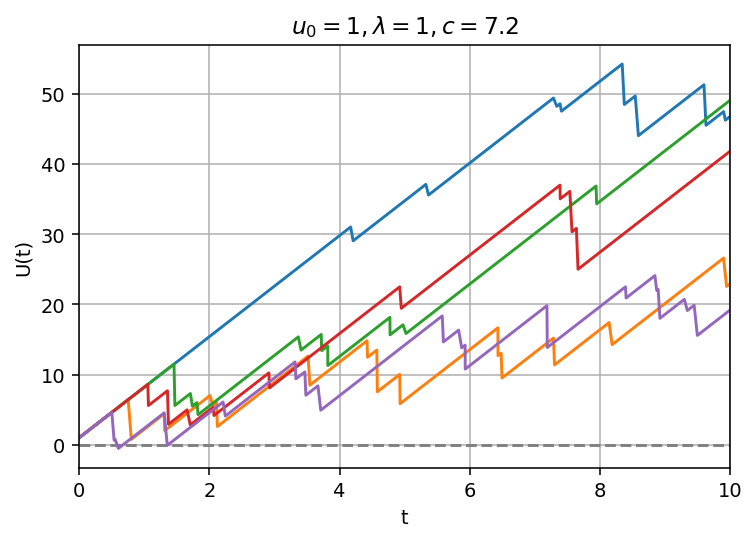
\includegraphics{traj_1.png}


    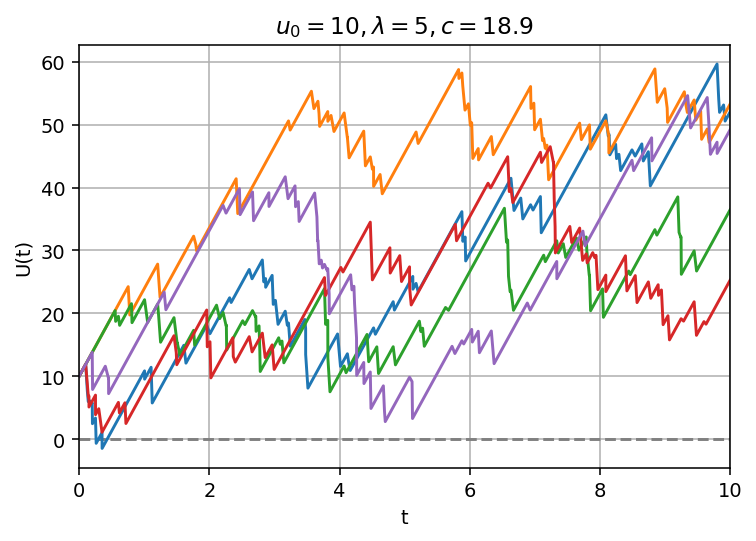
\includegraphics{traj_2.png}

    \section{Грубий метод Монте-Карло}

    Змоделювавши 1000 траекторій процесу $U$ для першого випадку ($u_0 = 1$, $\lambda = 1$ та $c = 7.2$) 
    отримали, що 421 з 1000 траекторій процесу збанкротували на цьому проміжку. Маємо оцінку ймовірності 
    банкрутства $p^*_1 =  0.421$.


    Змоделювавши 1000 траекторій процесу $U$ для другого випадку ($u_0 = 10$, $\lambda = 5$ та $c = 18.9$) 
    отримали, що 768 з 1000 траекторій процесу збанкротували на цьому проміжку. Маємо оцінку ймовірності 
    банкрутства $p^*_1 =  0.768$.


    Результати обрахунків можна побачити на скріншоті нижче:

    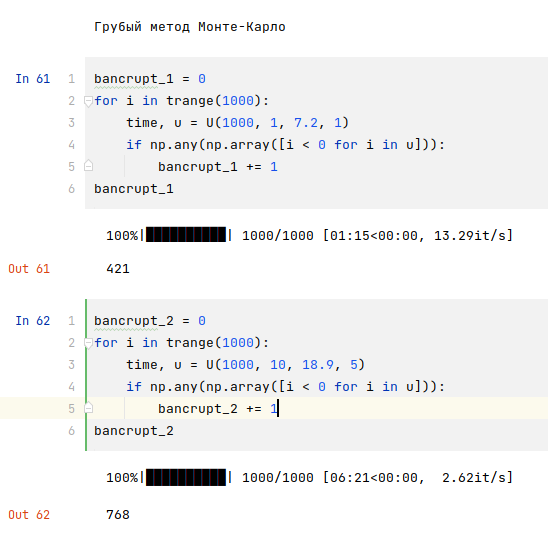
\includegraphics[scale=0.52]{img/2021-10-11-01-29-11.png}

    \section{Більш точний метод Монте-Карло}

    Оцiнити ймовiрнiсть банкрутства за допомогою бiльш точного методу Монте-Карло: 
    для цього спочатку записати функцiю розподiлу модифiкованої величини $\hat{X}$, 
    а потiм змоделювати геометрично розподiлену кiлькiсть незалежних копiй цiєї величини.

    Згідно з лекційному матеріалу функція розподілу $\hat{X}$ має вигляд 
    \begin{gather}
        F_{\hat{X}}(x) = \frac{1}{\E X} \intl_0^x(1 - F_X(y))dy
    \end{gather}

    Вираз для $1 - F_X(y)$ було знайдено раніше, запишемо функцію розподілу:
    \begin{gather}
        F_{\hat{X}}(x) = 
        \begin{cases}
            0, & x < 0\\
            \frac{1}{3.6}\intl_0^x 1dy = \frac{10x}{36}, & 0 \leq x < 1 \\
            \frac{1}{3.6}(\intl_0^1 1dy +\intl_1^x \frac{6-y}{5}dy) = \frac{-x^2 + 12x - 1}{36},& 1 \leq x < 5 \\
            \frac{1}{3.6}(\intl_0^1 1dy +\intl_1^5 \frac{6-y}{5}dy +\intl_5^x 0.2dy) = \frac{34 + 2(x-5)}{36},& 5 \leq x < 6 \\
            \frac{1}{3.6}(\intl_0^1 1dy +\intl_1^5 \frac{6-y}{5}dy +\intl_5^6 0.2dy) = 1,& x \geq 6
        \end{cases}
    \end{gather}
    Записавши функцiю розподілу - можемо записати і обернену функцію:
    \begin{gather}
        F^{-1}_{\hat{X}} (y) = 
        \begin{cases}
            3.6y, & y \in [0, \frac{10}{36}) \\
            6 - \sqrt{35 - 36y}, & y \in [\frac{10}{36}, \frac{34}{36}) \\
            18y - 12, & y \in [\frac{34}{36}, 1)
        \end{cases}
    \end{gather}
    За допомогою оберненої функції розподілу зможемо змоделювати цю випадкову величину.

    Згідно лекційного матеріалу запишемо формулу ймовірності банкрутства:
    \begin{gather}
        \psi(u) = 1 - \varphi(u) = 1 - \P\{\suml_{i=1}^G\hat{X_i} \leq u_0\} = \P\{\suml_{i=1}^G\hat{X_i} > u_0\}
    \end{gather}
    $u_0$ -- стартовий капітал, $G \sim Geom(1 - \frac{\lambda\mu}{c})$.
    Змоделюємо 1000 реалізацій $G$ окремо для першого та другого випадку та для кожної з реалізацій $G^*$ змоделюємо 
    відповідну сумму $\suml_{i=1}^{G^*}\hat{X_i}$. 

    Для першого випадку ($u_0 = 1$, $\lambda = 1$ та $c = 7.2$) 
    отримали оцінку ймовірності на проміжку $[0, 1000]$
    банкрутства $p^*_1 =  0.413$.

    Для другого випадку ($u_0 = 10$, $\lambda = 5$ та $c = 18.9$) 
    отримали оцінку ймовірності на проміжку $[0, 1000]$
    банкрутства $p^*_2 =  0.892$.


    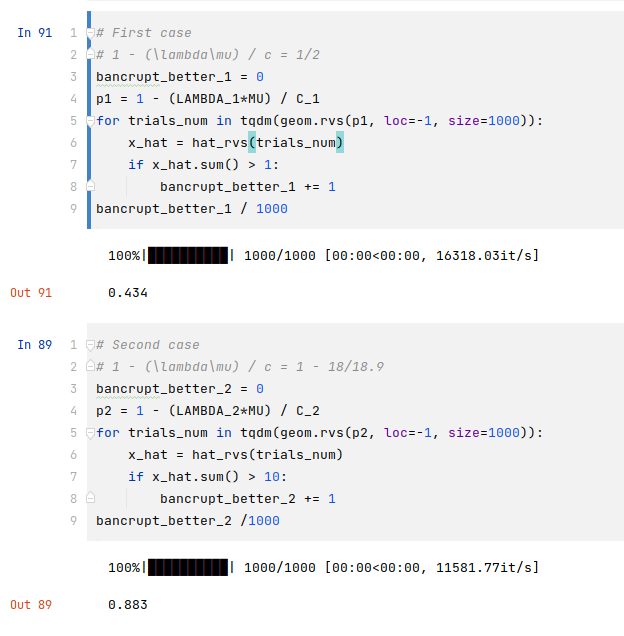
\includegraphics[scale=0.5]{img/2021-10-11-18-56-31.png}

    \section{Знаходження оберненого перетворення Лапласа}

    Знайшовши обернене перетворення Лапласа від $\Phi_1(p)$ та $\Phi_2(p)$ 
    - отримаємо функції $\varphi_1(u)$ та $\varphi_2(u)$ в які підставимо відповідні початкові умови та 
    отримаємо ймовiрнiсть банкрутства як $\psi^*_1 = 1 - \varphi_1(u_0)$ та $\psi^*_2 = 1 - \varphi_2(u_0)$.

    Після чисельного знаходження оберненого перетворення Лапласа отримано результати 
    $\psi^*_1 = 0.434$ та $\psi^*_2 = 0.883$.

    Результати можна побачити нижче.

    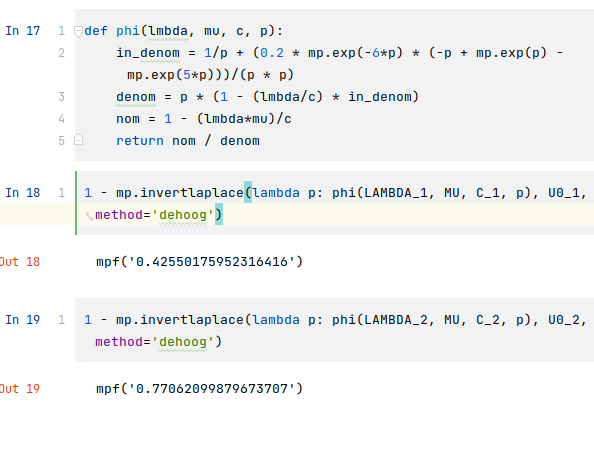
\includegraphics[scale=0.5]{img/2021-10-11-17-27-01.png}

    \section{Висновки}

    В таблиці нижче приведені результати досліджень:

    \begin{tabular}{@{}|l|l|l|@{}}
    \toprule
    Грубий ММК & Більш точний ММК & Обернене перетворення Лапласа \\ \midrule
    \multicolumn{3}{|c|}{$\lambda = 1$, $u_0 = 1$, $c = 7.2$}       \\\hline
    0.421      & 0.434            & 0.426                         \\\hline
    \multicolumn{3}{|c|}{$\lambda = 5$, $u_0 = 10$, $c = 18.9$}     \\\hline
    0.768      & 0.883            & 0.771                         \\ \bottomrule
    \end{tabular}

    
    В ході роботи було розглянуто три методи підрахунку ймовірності банкрутства: два ММК та за 
    допомогою знаходження оберненого перетворення Лапласа. 


    Грубий метод ММК є дуже ресурсозатратним (т.я. на кожній ітерації необхідно отримати траекторію 
    процеса страхового ризику). В силу обчислювальної складності моделювання самого процесу 
    виникає проблема, що навіть при виборці в 1000 траекторій грубий ММК відпрацьовує в залежності 
    від параметрів від 2 до 4 хвилин на відміну від більш точного методу МНК. Зрозуміло, що 
    <<точний>> метод МНК буде мати більш наближені до дійсності результати в силу того, що 
    він враховує увесь проміжок $[0, \infty)$, а не тільки $[0, 1000)$ як перший метод в силу 
    своєї побудови. З іншого боку <<точний>> метод МНК є більш аналітично складним і потребує 
    попередню підготовку до моделювання у вигляді знаходження функції розподілу величин $\hat{X}$. 


    Хочется зазначити, що обидва з методів Монте-Карло при розмірі виборки в 1000 елементів є 
    достатньо мінливими. Значення оцінок ймовірності можуть суттєво змінюватись при різних 
    запусках обох методів. Якщо ж взяти вибірку в $10^6$ елементів -- справи стають набагато краще 
    (можемо бачити на прикладі нижче).

    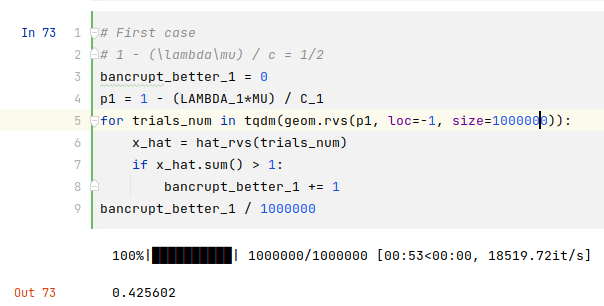
\includegraphics[scale=0.5]{img/2021-10-11-18-53-04.png}

    В такому разі результати обох методів стають набагато ближче до найкращого з методів - 
    використання оберненого перетворення Лапласа. За допомогою цього метода ми можемо:
    \begin{itemize}
        \item у деяких 
        випадках навіть знайти функцiю $\varphi(u)$ аналітично (дуже рідкі такі випадки, 
        але ймовiрнiсть така є);
        \item коли не можемо знайти аналітично (практично завжди) -- можемо застосувати 
        чисельні методи обчислення оберненого перетворення Фур'є, для яких ми не тільки можемо 
        задати точність виконання, а й за допомогою отриманих результатів інтерполювати функцiю 
        $\varphi(u)$ і таким чином зрозуміти залежність між початковим капіталом та ймовiрнiстю 
        небанкрустства;
    \end{itemize}
    
\end{document}